\documentclass[border=16pt]{standalone}
\usepackage{tikz}
\usetikzlibrary{shapes,arrows.meta,positioning,calc}
\renewcommand{\familydefault}{\sfdefault}

\begin{document}
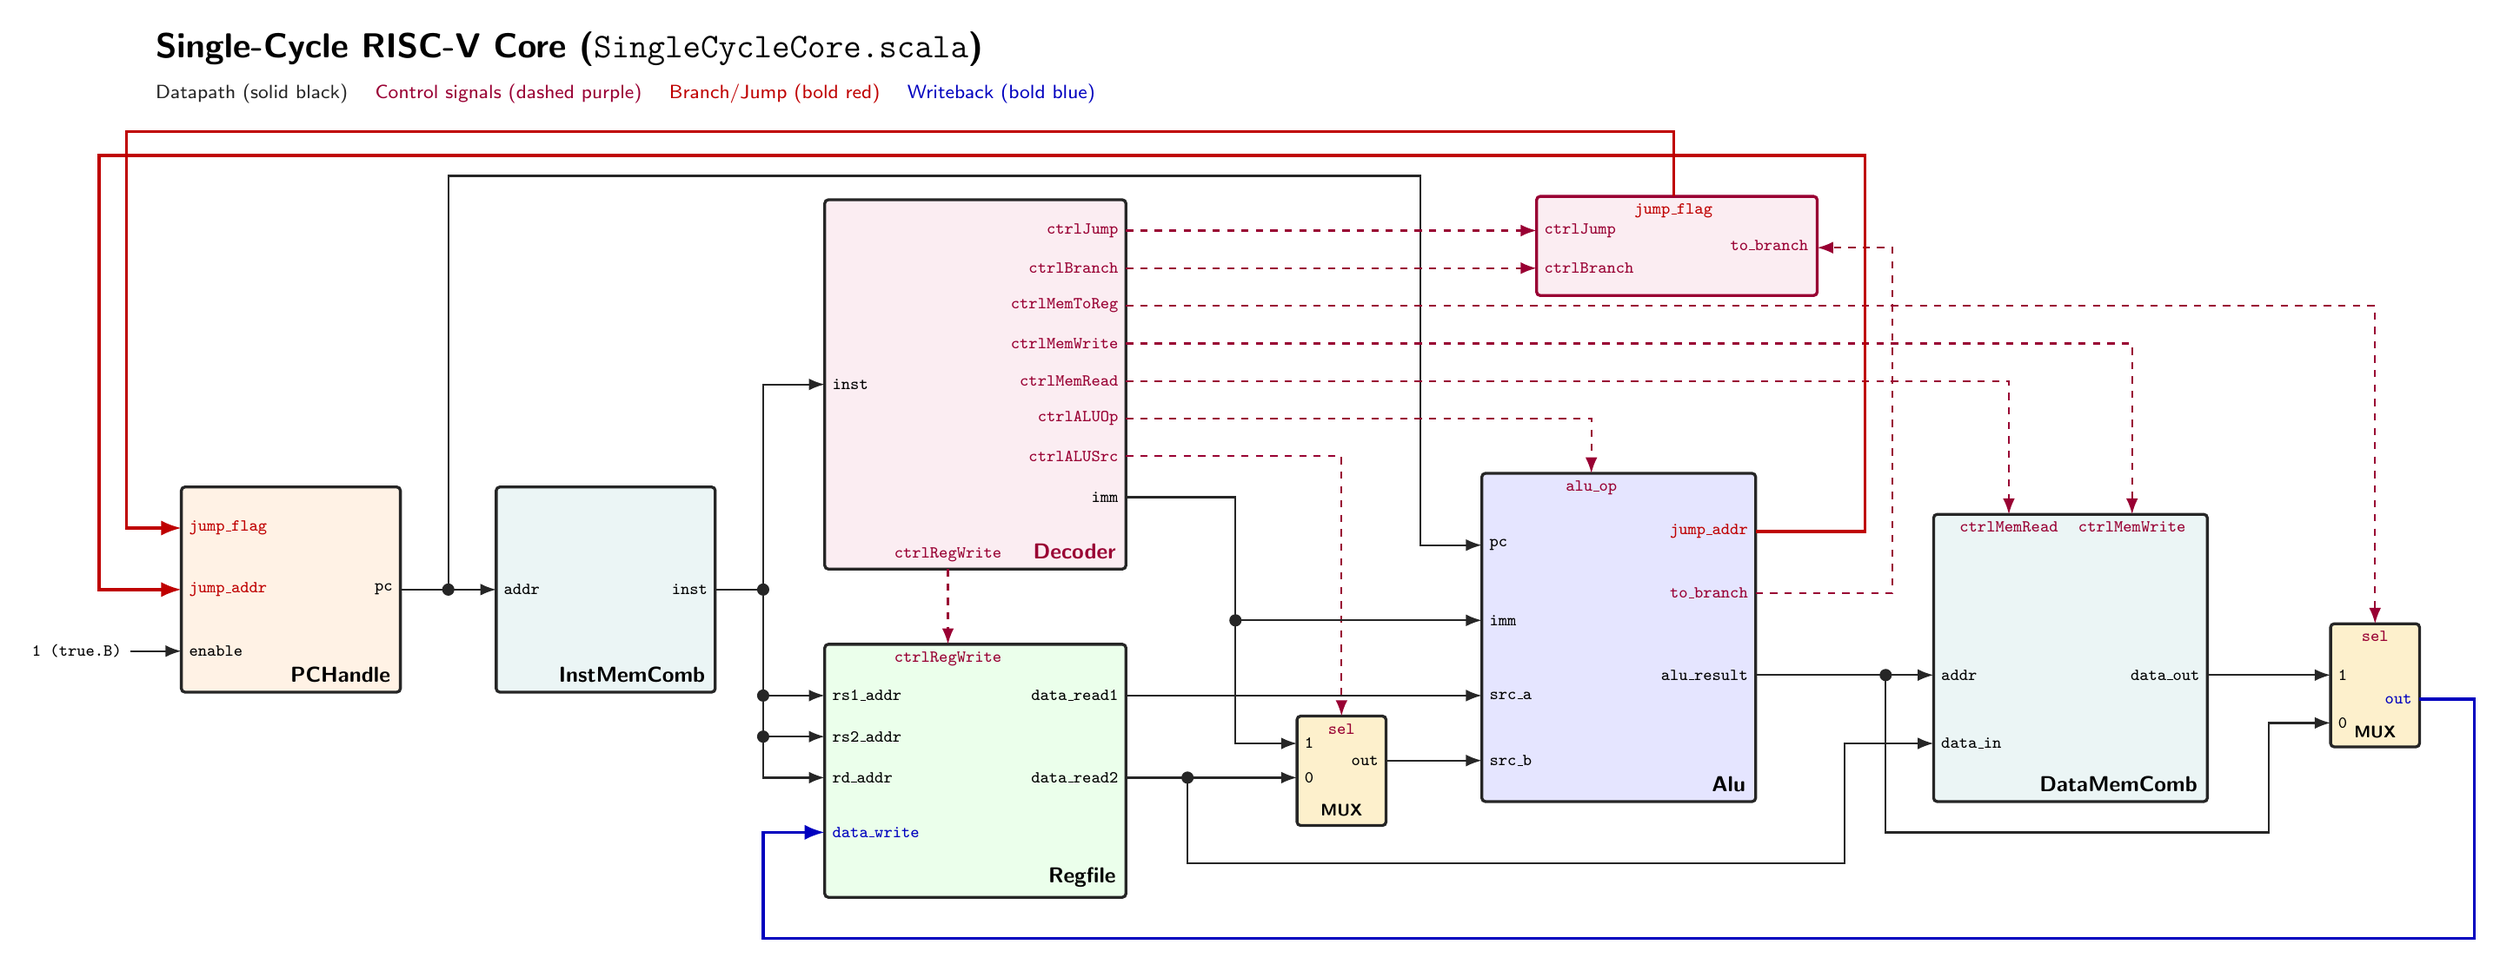
\begin{tikzpicture}[
    >=Latex,
    font=\scriptsize,
    box/.style={draw=black!85, very thick, fill=white, rounded corners=1.5pt},
    pinL/.style={anchor=west, font=\scriptsize\ttfamily, inner sep=3pt},
    pinR/.style={anchor=east, font=\scriptsize\ttfamily, inner sep=3pt},
    pinT/.style={anchor=north, font=\scriptsize\ttfamily, inner sep=3pt},
    pinB/.style={anchor=south, font=\scriptsize\ttfamily, inner sep=3pt},
    modtitle/.style={anchor=south east, font=\small\bfseries, inner sep=4pt},
    wire/.style={->, thick, draw=black!85},
    cwire/.style={->, thick, draw=purple!80!black, dashed},
    bwire/.style={->, very thick, draw=red!75!black},
    wbwire/.style={->, very thick, draw=blue!75!black},
    lbl/.style={font=\scriptsize\ttfamily, inner sep=2pt},
    dot/.style={circle, fill=black!85, inner sep=1.8pt}
]
\definecolor{amber}{RGB}{245,180,0}

% Title
\node[font=\Large\bfseries, anchor=west] at (-1.5, 9.6) {Single-Cycle RISC-V Core (\texttt{SingleCycleCore.scala})};
\node[font=\footnotesize, anchor=west] at (-1.5, 8.95) {\textcolor{black!85}{Datapath (solid black)} \quad \textcolor{purple!80!black}{Control signals (dashed purple)} \quad \textcolor{red!75!black}{Branch/Jump (bold red)} \quad \textcolor{blue!75!black}{Writeback (bold blue)}};

% =========================================================================
% 1. PCHandle (x: -1.0 .. 2.2, y: 0.2 .. 3.2)
% =========================================================================
\draw[box, fill=orange!10] (-1.0, 0.2) rectangle (2.2, 3.2);
\node[pinL, text=red!75!black] at (-1.0, 2.6) {jump\_flag};
\node[pinL, text=red!75!black] at (-1.0, 1.7) {jump\_addr};
\node[pinL]                    at (-1.0, 0.8) {enable};
\node[pinR]                    at (2.2, 1.7) {pc};
\node[modtitle] at (2.2, 0.2) {PCHandle};

\node[font=\scriptsize, align=right, anchor=east] (trueb) at (-1.75, 0.8) {\texttt{1 (true.B)}};
\draw[wire] (-1.75, 0.8) -- (-1.0, 0.8);

% =========================================================================
% 2. InstMemComb (x: 3.6 .. 6.8, y: 0.2 .. 3.2)
% =========================================================================
\draw[box, fill=teal!8] (3.6, 0.2) rectangle (6.8, 3.2);
\node[pinL] at (3.6, 1.7) {addr};
\node[pinR] at (6.8, 1.7) {inst};
\node[modtitle] at (6.8, 0.2) {InstMemComb};

% =========================================================================
% 3. Decoder (x: 8.4 .. 12.8, y: 2.0 .. 7.4)
% =========================================================================
\draw[box, fill=purple!7] (8.4, 2.0) rectangle (12.8, 7.4);
\node[pinL] at (8.4, 4.7) {inst};

% Right-side output pins of Decoder (strictly ordered top to bottom so wires never cross!)
\node[pinR, text=purple!80!black] at (12.8, 6.95) {ctrlJump};
\node[pinR, text=purple!80!black] at (12.8, 6.40) {ctrlBranch};
\node[pinR, text=purple!80!black] at (12.8, 5.85) {ctrlMemToReg};
\node[pinR, text=purple!80!black] at (12.8, 5.30) {ctrlMemWrite};
\node[pinR, text=purple!80!black] at (12.8, 4.75) {ctrlMemRead};
\node[pinR, text=purple!80!black] at (12.8, 4.20) {ctrlALUOp};
\node[pinR, text=purple!80!black] at (12.8, 3.65) {ctrlALUSrc};
\node[pinR]                       at (12.8, 3.05) {imm};

% Bottom output pin of Decoder
\node[pinB, text=purple!80!black] at (10.2, 2.0) {ctrlRegWrite};
\node[modtitle, text=purple!80!black] at (12.8, 2.0) {Decoder};

% =========================================================================
% 4. Regfile (x: 8.4 .. 12.8, y: -2.8 .. 0.9) -- Textbook Port Style!
% =========================================================================
\draw[box, fill=green!8] (8.4, -2.8) rectangle (12.8, 0.9);
\node[pinT, text=purple!80!black] at (10.2, 0.9) {ctrlRegWrite};
\node[pinL]                       at (8.4, 0.15)  {rs1\_addr};
\node[pinL]                       at (8.4, -0.45) {rs2\_addr};
\node[pinL]                       at (8.4, -1.05) {rd\_addr};
\node[pinL, text=blue!75!black]   at (8.4, -1.85) {data\_write};
\node[pinR] at (12.8, 0.15) {data\_read1};
\node[pinR] at (12.8, -1.05){data\_read2};
\node[modtitle] at (12.8, -2.8) {Regfile};

% =========================================================================
% 5. ALUSrc MUX (x: 15.3 .. 16.6, y: -1.75 .. -0.15)
% =========================================================================
\draw[box, fill=amber!20] (15.3, -1.75) rectangle (16.6, -0.15);
\node[pinT, text=purple!80!black] at (15.95, -0.15) {sel};
\node[pinL] at (15.3, -0.55) {1};
\node[pinL] at (15.3, -1.05) {0};
\node[pinR] at (16.6, -0.80) {out};
\node[font=\scriptsize\bfseries] at (15.95, -1.52) {MUX};

% =========================================================================
% 6. Alu (x: 18.0 .. 22.0, y: -1.4 .. 3.4)
% =========================================================================
\draw[box, fill=blue!10] (18.0, -1.4) rectangle (22.0, 3.4);
\node[pinT, text=purple!80!black] at (19.6, 3.4) {alu\_op};
\node[pinL] at (18.0, 2.35) {pc};
\node[pinL] at (18.0, 1.25) {imm};
\node[pinL] at (18.0, 0.15) {src\_a};
\node[pinL] at (18.0, -0.80){src\_b};
\node[pinR, text=red!75!black]    at (22.0, 2.55) {jump\_addr};
\node[pinR, text=purple!80!black] at (22.0, 1.65) {to\_branch};
\node[pinR]                       at (22.0, 0.45) {alu\_result};
\node[modtitle] at (22.0, -1.4) {Alu};

% =========================================================================
% 7. Branch / Jump Gate (x: 18.8 .. 22.9, y: 6.0 .. 7.45)
% =========================================================================
\draw[box, fill=purple!7, draw=purple!80!black] (18.8, 6.0) rectangle (22.9, 7.45);
\node[pinL, text=purple!80!black] at (18.8, 6.95) {ctrlJump};
\node[pinL, text=purple!80!black] at (18.8, 6.40) {ctrlBranch};
\node[pinB, text=purple!80!black] at (22.2, 6.55)  {to\_branch};
\node[pinT, text=red!75!black]    at (20.8, 7.45) {jump\_flag};

% =========================================================================
% 8. DataMemComb (x: 24.6 .. 28.6, y: -1.4 .. 2.8)
% =========================================================================
\draw[box, fill=teal!8] (24.6, -1.4) rectangle (28.6, 2.8);
\node[pinT, text=purple!80!black] at (25.7, 2.8) {ctrlMemRead};
\node[pinT, text=purple!80!black] at (27.5, 2.8) {ctrlMemWrite};
\node[pinL] at (24.6, 0.45) {addr};
\node[pinL] at (24.6, -0.55){data\_in};
\node[pinR] at (28.6, 0.45) {data\_out};
\node[modtitle] at (28.6, -1.4) {DataMemComb};

% =========================================================================
% 9. MemToReg MUX (x: 30.4 .. 31.7, y: -0.6 .. 1.2)
% =========================================================================
\draw[box, fill=amber!20] (30.4, -0.6) rectangle (31.7, 1.2);
\node[pinT, text=purple!80!black] at (31.05, 1.2) {sel};
\node[pinL]                       at (30.4, 0.45) {1};
\node[pinL]                       at (30.4, -0.25){0};
\node[pinR, text=blue!75!black]   at (31.7, 0.10) {out};
\node[font=\scriptsize\bfseries] at (31.05, -0.38) {MUX};

% =========================================================================
% WIRES & CONNECTIONS (All T-junctions have explicit black dots!)
% =========================================================================
% 1. PC -> InstMemComb & Alu
\draw[wire] (2.2, 1.7) -- (3.6, 1.7);
\node[dot] at (2.9, 1.7) {};
\draw[wire] (2.9, 1.7) -- (2.9, 7.75) -- (17.1, 7.75) |- (18.0, 2.35);

% 2. InstMemComb -> Decoder & Regfile (with all 3 T-junction black dots!)
\draw[wire] (6.8, 1.7) -- (7.5, 1.7) |- (8.4, 4.7);
\node[dot] at (7.5, 1.7) {};
\draw[wire] (7.5, 1.7) -- (7.5, -1.05) -- (8.4, -1.05);
\node[dot] at (7.5, 0.15) {};
\draw[wire] (7.5, 0.15) -- (8.4, 0.15);
\node[dot] at (7.5, -0.45) {};
\draw[wire] (7.5, -0.45) -- (8.4, -0.45);

% 3. Decoder -> Regfile (ctrlRegWrite)
\draw[cwire] (10.2, 2.0) -- (10.2, 0.9);

% 4. Decoder -> Control Signals
\draw[cwire] (12.8, 6.95) -- (18.8, 6.95);
\draw[cwire] (12.8, 6.40) -- (18.8, 6.40);
\draw[cwire] (12.8, 5.85) -| (31.05, 1.2);
\draw[cwire] (12.8, 5.30) -| (27.5, 2.8);
\draw[cwire] (12.8, 4.75) -| (25.7, 2.8);
\draw[cwire] (12.8, 4.20) -| (19.6, 3.4);
\draw[cwire] (12.8, 3.65) -| (15.95, -0.15);

% 5. Decoder -> imm (to Alu and ALUSrc MUX, with T-junction black dot!)
\draw[wire] (12.8, 3.05) -- (14.4, 3.05) |- (15.3, -0.55);
\node[dot] at (14.4, 1.25) {};
\draw[wire] (14.4, 1.25) -- (18.0, 1.25);

% 6. Regfile -> Alu, ALUSrc MUX, DataMemComb (with T-junction black dot!)
\draw[wire] (12.8, 0.15) -- (18.0, 0.15);
\draw[wire] (12.8, -1.05) -- (15.3, -1.05);
\node[dot] at (13.7, -1.05) {};
\draw[wire] (13.7, -1.05) -- (13.7, -2.3) -- (23.3, -2.3) |- (24.6, -0.55);

% 7. ALUSrc MUX -> Alu.src_b
\draw[wire] (16.6, -0.80) -- (18.0, -0.80);

% 8. Alu -> Branch Gate, DataMemComb, MemToReg MUX (with T-junction black dot!)
\draw[cwire] (22.0, 1.65) -- (24.0, 1.65) -- (24.0, 6.70) -- (22.9, 6.70);
\draw[wire] (22.0, 0.45) -- (24.6, 0.45);
\node[dot] at (23.9, 0.45) {};
\draw[wire] (23.9, 0.45) -- (23.9, -1.85) -- (29.5, -1.85) |- (30.4, -0.25);

% 9. DataMemComb -> MemToReg MUX
\draw[wire] (28.6, 0.45) -- (30.4, 0.45);

% 10. Branch Gate & Alu.jump_addr -> PCHandle (Red)
\draw[bwire] (20.8, 7.45) -- (20.8, 8.4) -- (-1.8, 8.4) |- (-1.0, 2.6);
\draw[bwire] (22.0, 2.55) -- (23.6, 2.55) -- (23.6, 8.05) -- (-2.2, 8.05) |- (-1.0, 1.7);

% 11. MemToReg MUX -> Regfile.data_write (Blue Writeback)
\draw[wbwire] (31.7, 0.10) -- (32.5, 0.10) -- (32.5, -3.4) -- (7.5, -3.4) |- (8.4, -1.85);

\end{tikzpicture}
\end{document}
